\section{Consuntivo}\label{Consuntivi}
Verranno di seguito riportate le spese effettivamente sostenute, che saranno poi confrontate con quelle preventivate al fine di presentare un bilancio. \\
Il bilancio sarà:
\begin{itemize}
\item \textbf{Positivo:} se il preventivo supera il consuntivo;
\item \textbf{Negativo:} se il consuntivo supera il preventivo;
\item \textbf{In pari:} se il consuntivo e il preventivo corrispondono.
\end{itemize}
%\subsection{Consuntivo fase di Analisi}
%Si riporta di seguito il consuntivo della fase di \fA, il bilancio di questa fase viene riportato solamente a scopo informativo, in quanto le spese sostenute in questa fase sono a carico del \gloxy{fornitore}.\\
%%tabella costi
%\begin{table}[h]
%\begin{center}
%\begin{tabular}{|m{3cm}|m{1.5cm}|m{1.5cm}|}
%\hline Ruolo & Ore & Costo (\euro) \\
%\hline
%\rRPt & -4 & -120 \\
%\rAPt & 0 & 0 \\
%\rAt & 0 & 0 \\
%\rPt & 0 & 0 \\
%\rpt & 0 & 0 \\
%\rVt & +4 & +60 \\
%\hline
%Totale & 0 & -60 \\
%\hline
%\end{tabular}
%\caption{Differenza consuntivo e preventivo - Fase di \fAt}
%\end{center}
%\end{table}
%\FloatBarrier
%\subsubsection{Conclusioni}
%La pianificazione delle varie attività si è rilevata essere corretta per quasi tutte le attività, fanno però eccezione le attività legate all'analisi dei requisiti che hanno subito uno slittamento in avanti dovuto ad un periodo di inattività non previsto durante il periodo delle vacanze Natalizie.\\
%Questo slittamento in avanti è andato ad occupare i giorni di \gloxy{slack} che erano stati appositamente pianificati inoltre, come si può notare dalla tabella, trattandosi di uno slittamento, non è stato necessario aumentare le ore di lavoro.\\
%%Come si può notare dalla tabella, sono state preventivate più ore di \rA rispetto a quelle necessarie, che ha portato un risparmio di \textbf{132\euro}.\\
%Sono state invece sovrastimate le ore di lavoro del \rRP che ha lavorato 4 ore in meno, portando ad un risparmio di 120\euro.\\
%Queste 4 ore che si sono liberate sono state utilizzate per ulteriori attività di verifica, portando ad un risparmio complessivo di \textbf{60\euro}.\\
%Si ricorda che questo bilancio è puramente indicativo in quanto le fasi di \fA e \fAD sono a carico del \gloxy{fornitore}.
\subsection{Consuntivo di periodo -\fPAt}\label{CfPA}
%\subsubsection{Consuntivo di periodo}
Viene indicata la differenza tra il preventivo calcolato in §\ref{prospettofPAt} e le spese effettive sostenute durante questa fase.
%tabella costi
\begin{table}[h]
\begin{center}
\begin{tabular}{|m{3cm}|m{1.5cm}|m{1.5cm}|}
\hline Ruolo & Ore & Costo (\euro) \\
\hline
\rRPt & 0 & 0 \\
\rAPt & 0 & 0 \\
\rAt & -3 & -75 \\
\rPt & 0 & 0 \\
\rpt & 0 & 0 \\
\rVt & +3 & +45 \\
\hline
Totale & 0 & -30\euro \\
\hline
\end{tabular}
\caption{Differenza tra preventivo e consuntivo - Fase di \fPAt}
\end{center}
\end{table}
\FloatBarrier
\subsubsection{Conclusioni}
Grazie all'incremento del documento \NP, eseguito scrupolosamente durante la precedente fase di \fAD, non è stato necessario impiegare la maggior parte delle ore antecedentemente destinate al ruolo di \rAP. Le ore risparmiate sono state impiegate in tre ore aggiuntive per la verifica dei documenti incrementati.
%In questa fase non è stato possibile risparmiare sui costi preventivati in quanto si sono verificati alcuni rischi che hanno consumato i margini precedentemente preventivati per la fase stessa.
\subsection{Consuntivo di periodo - \fPDt}\label{CfPD}
%\subsubsection{Consuntivo di periodo}\label{consuntivoDP}
Viene indicata la differenza tra il preventivo calcolato in §\ref{prospettofPDt} e le spese effettive sostenute durante questa fase.
%Tabella costi
\begin{table}[h]
\begin{center}
\begin{tabular}{|m{3cm}|m{1.5cm}|m{1.5cm}|}
\hline Ruolo & Ore & Costo (\euro) \\
\hline
\rRPt & 0 & 0 \\
\rAPt & -2 & -40 \\
\rAt & 0 & 0 \\
\rPt & +2 & +44 \\
\rpt & 0 & 0 \\
\rVt & 0 & 0 \\
\hline
Totale & 0 & +4\euro \\
\hline
\end{tabular}
\caption{Differenza tra preventivo e consuntivo - Fase di \fPDt}
\end{center}
\end{table}
\FloatBarrier
\subsubsection{Conclusioni}\label{conclusioniDP}
Grazie all'ottima implementazione degli strumenti di lavoro, effettuata nelle fasi precedenti, sono state necessarie meno ore di quelle preventivate per la manutenzione e l'aggiornamento delle stesse in vista della definizione dell'architettura.
Tuttavia le ore risparmiate sono state impiegate per rifinire e corregge alcuni problemi legati alla progettazione dell'architettura, emersi prima dell'effettivo consolidamento della stessa.\\
% Aggiunta per i test
Nonostante le due ore extra di lavoro da parte dei \rPs non è stato possibile definire anche i test d'unità per le varie componenti progettate in questa fase. \`E stato scelto di non aumentare le ore di lavoro per i \rPs dal momento che per la fase \fC sono pianificate 40 ore da destinare a questo ruolo, parte delle quali verranno utilizzate per definire i test mancanti. \\
Questa nuova suddivisone è possibile perché parte delle ore preventivate per le correzioni e la manutenzione del documento di \ST possono essere riassegnate. Infatti la \ST è rimasto un documento interno e informale, quindi sarà necessaria una manutenzione minore.
% Inoltre i pareri dei committenti, espressi in vari incontri, sembrano indicare che l'architettura generale proposta soddisfi le aspettative del prodotto.
%In questa fase non è stato possibile risparmiare sui costi preventivati in quanto si sono verificati alcuni rischi che hanno consumato i margini precedentemente preventivati per la fase stessa.
\subsection{Consuntivo di periodo - \fCt}\label{CfC}
%\subsubsection{Consuntivo di periodo}\label{consuntivoCod}
Viene indicata la differenza tra il preventivo calcolato in §\ref{prospettoCod} e le spese effettive sostenute durante questa fase.
%Tabella costi
\begin{table}[h]
\begin{center}
\begin{tabular}{|m{3cm}|m{1.5cm}|m{1.5cm}|}
\hline Ruolo & Ore & Costo (\euro) \\
\hline
\rRPt & +1 & +30 \\
\rAPt & 0 & 0 \\
\rAt & -4 & -100 \\
\rPt & 0 & 0 \\
\rpt & +1 & +15 \\
\rVt & 0 & 0 \\
\hline
Totale & -2 & -55\euro \\
\hline
\end{tabular}
\caption{Differenza tra preventivo e consuntivo - Fase di \fCt}
\end{center}
\end{table}
\FloatBarrier
\subsubsection{Conclusioni}\label{conclusioniFC}
A conclusione del periodo trascorso ci sono state alcune variazioni per quanto riguarda quanto pianificato in \ref{prospettoCod}.\newline
Visto l'ottimo esito del documento di \AR e la mancata variazione dei requisiti, è stato possibile ridurre in modo sostanziale le ore da \rA.\newline
I soldi recuperati da questo taglio hanno permesso un reinvestimento in altri ruoli.\newline
In primo luogo si è deciso di aumentare le ore del \rRP.\newline
Questo aumento è stato causato dagli errori di bilancio riscontrati nel \PP, che hanno richiesto una ripianificazione dei preventivi, dei costi e delle ore al fine di rientrare nella somma proposta al \gloxy{Committente}.\newline
In seguito è stato necessario un aumento delle ore da \rp, poiché sono sorti degli imprevisti nell'integrazione dei moduli \gloxy{back-end} e \gloxy{front-end} dell'applicativo, che hanno richiesto più impegno di quanto stimato. Tuttavia si sono trattate di problematiche rapidamente risolvibili.\newline
In conclusione, il risparmiato per questa fase è stato di \textbf{\euro55} e sono state rendicontate due ore di lavoro in meno del previsto.\newline
In un primo momento si era pensato di reinvestire nell'immediato i soldi risparmiati in attività di verifica ma, visto che per questa fase la sua percentuale risulta buona, si è deciso di conservarli in ottica della \fVV con le motivazioni che verranno trattate di seguito.
Visti i rischi preventivati, è possibile che siano richieste più ore da \rRP per mitigare i contrasti interni fra i membri del \gloxy{team}. Inoltre, si assume che ci possano volere più ore di codifica per implementare le funzionalità finali dell'applicativo. Nel caso tali ipotesi non si verificassero è comunque lecito assumere che le ore vengano investite in verifica.
In conclusione si è risparmiato per questa fase un totale di \textbf{\euro55} e sono state rendicontate due ore di lavoro in meno del previsto.\newline
\subsection{Consuntivo di periodo - \fVV}\label{CfVV}
%\subsubsection{Consuntivo di periodo}\label{consuntivoVer}
Viene indicata la differenza tra il preventivo calcolato in §\ref{prospettoVer} e le spese effettive sostenute durante questa fase.
%Tabella costi
\begin{table}[h]
\begin{center}
\begin{tabular}{|m{3cm}|m{1.5cm}|m{1.5cm}|}
\hline Ruolo & Ore & Costo (\euro) \\
\hline
\rRPt & -1 & -30 \\
\rAPt & 0 & 0 \\
\rAt & 0 & 0 \\
\rPt & 0 & 0 \\
\rpt & +4 & +60 \\
\rVt & +1 & +15 \\
\hline
Totale & +2 & +45\euro \\
\hline
\end{tabular}
\caption{Differenza tra preventivo e consuntivo - Fase di \fVV}
\end{center}
\end{table}
\FloatBarrier
\subsubsection{Conclusioni}\label{conclusioniFC}
A conclusione del periodo trascorso ci sono state alcune variazioni per quanto riguarda quanto pianificato in §\ref{prospettoVer}.\newline
Durante questa fase di lavoro si sono presentate alcune leggere problematiche che hanno richiesto delle azioni di correzione per quanto riguarda la distribuzione delle ore di lavoro.
Il flusso di lavoro è organizzato in maniera ottimale e i membri del \gloxy{team} riescono ad autogestirsi per alcuni aspetti del lavoro richiesto.
Il sistema organizzativo impone scadenze ben precise e pesate che permettono di avere sempre sotto controllo lo stato dei lavori ed eventuali ritardi.
Per queste motivazioni il lavoro del \rRP è fortemente agevolato portando ad un risparmio di un ora lavorativa rispetto a quanto pianificato.\newline
A seguito di un incontro col il \gloxy{Proponente} il \gloxy{team} ha ricevuto delle indicazioni riguardo alcune migliorie grafiche da apportare all'applicativo con lo scopo di renderlo più accattivante e piacevole all'uso.
Questo lavoro non era stato preventivato e ha richiesto più tempo di quanto pianificato.
Il lavoro svolto non è stato oneroso e ha comunque permesso di mantenere le scadenze stabilite.
In totale sono state necessarie tre ore da \rRP per apportare quanto consigliato dal \gloxy{Proponente} e per apportare qualche miglioria ai test codificati durante questa ultima fase di lavoro.\newline
In conclusione il \gloxy{team} alla fine di questa fase ha avuto una spesa aggiuntiva di \euro45 rispetto a quanto preventivato.
\subsection{Consuntivo Finale}\label{CFinal}
In conclusione al \gloxy{progetto} sono state necessarie delle modifiche alle ore preventivate.
Di seguito vengono mostrate le variazioni in termini di ore e di costi sostenuti durante la realizzazione del \gloxy{progetto}.
\begin{table}[h]
\begin{center}
\begin{tabular}{|m{3cm}|m{3cm}|m{3cm}|m{1.5cm}|}
\hline Ruolo & Ore Preventivate & Ore Effettive &  Variazioni \\
\hline
\rRPt & 15 & 15 & 0 \\
\rAPt & 10 & 8 & -2 \\
\rAt & 15 & 8 & -7 \\
\rPt & 305 & 307 & +2 \\
\rpt & 128 & 133 & +5 \\
\rVt & 232 & 236 & +4 \\
\hline
Totale & 705 & 707 & +2\\
\hline
\end{tabular}
\caption{Variazione ore lavoro}
\end{center}
\end{table}
\FloatBarrier
A seguito delle variazioni riportate il carico di lavoro è leggermente variato rispetto a quanto preventivato.\\
Le ore effettive rendicontate svolte da i vari componenti del gruppo vengono riportate nella seguente tabella e riassunte nel successivo grafico.\\
\begin{table}[h]
\begin{center}
\begin{tabular}{|c|c|c|c|c|c|c|c|}
\hline Nome & Re & Am & An & Pt & Pr & Ve & Ore totali\\
\hline
\gma & - & 2 & 2 & 41 & 24 & 32 & 101 \\
\ao & - & - & - & 49 & 35 & 17 & 101 \\
\mb & 3 & - & 3 & 47 & 26 & 22 & 101 \\
\dm & 3 & - & - & 49 & 23 & 26 & 101 \\
\gmi & 6 & - & 1 & 34 & 6 & 54 & 101 \\
\sm & 3 & 4 & - & 51 & 10 & 33 & 101 \\
\fv & - & 2 & 2 & 36 & 9 & 52 & 101 \\
\hline Totale ruoli & 15 & 8 & 8 & 307 & 133 & 236 & 707 \\
\hline
\end{tabular}
\caption{Ore per componente - Effettive}
\end{center}
\end{table}
\FloatBarrier
\begin{figure}[htbp]
\centering
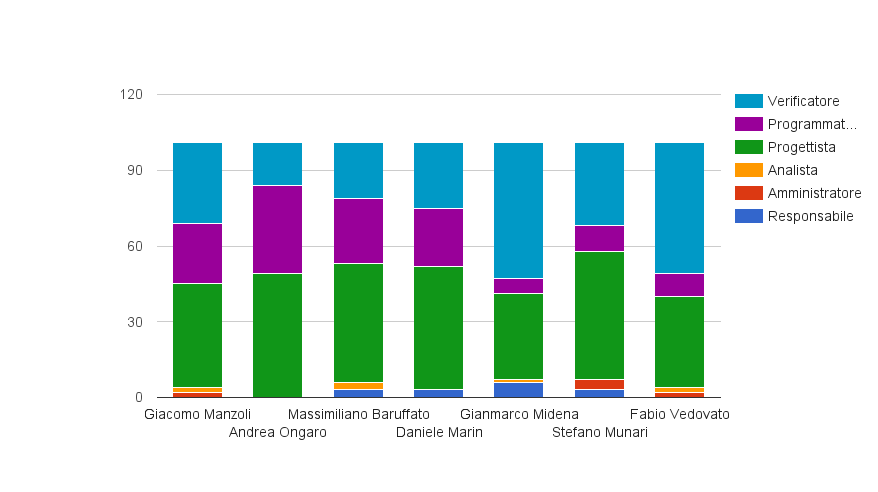
\includegraphics[width=\textwidth]{../immagini/nuoviGrafici/componenti/totaleOrePerRuoloFinali.png}
\caption{Ore per componente effettive}
\end{figure}
\FloatBarrier
Si ricorda che il vincolo di progetto riguardante il fatto che per tutta la durata del progetto didattico ogni componente deve svolgere ogni ruolo viene comunque soddisfatto, dal momento che la tabella sopra riportata non considera le ore d'investimento.
\subsubsection{Conclusioni}
Alla fine del \gloxy{progetto} il bilancio risulta \textbf{in positivo} di \textbf{\euro36} rispetto a quanto previsto.
Questo risparmio deriva dall'avanzo della fase precedente al quale si è sottratto la spesa avuta durante la fase di \fVV.
Essendo terminato il \gloxy{progetto} i soldi risparmiati comporteranno un abbassamento della quota stabilita con il \gloxy{committente} per la realizzazione del prodotto.\newline
Tale somma si aggiorna al totale di \textbf{\euro13.099}.
